\documentclass{article}

\usepackage{graphicx}
\usepackage{tikz}
\usepackage{tikzsymbols}
\usetikzlibrary{calc,patterns,shapes.geometric}
\pagestyle{empty}
\usepackage[margin=0pt]{geometry}
\geometry{papersize={14in,12in}}

\def\centerarc[#1](#2)(#3:#4:#5){\draw[#1] ($(#2)+({#5*cos(#3)},{#5*sin(#3)})$) arc (#3:#4:#5);}

\begin{document}
	\begin{figure}
		\centering
		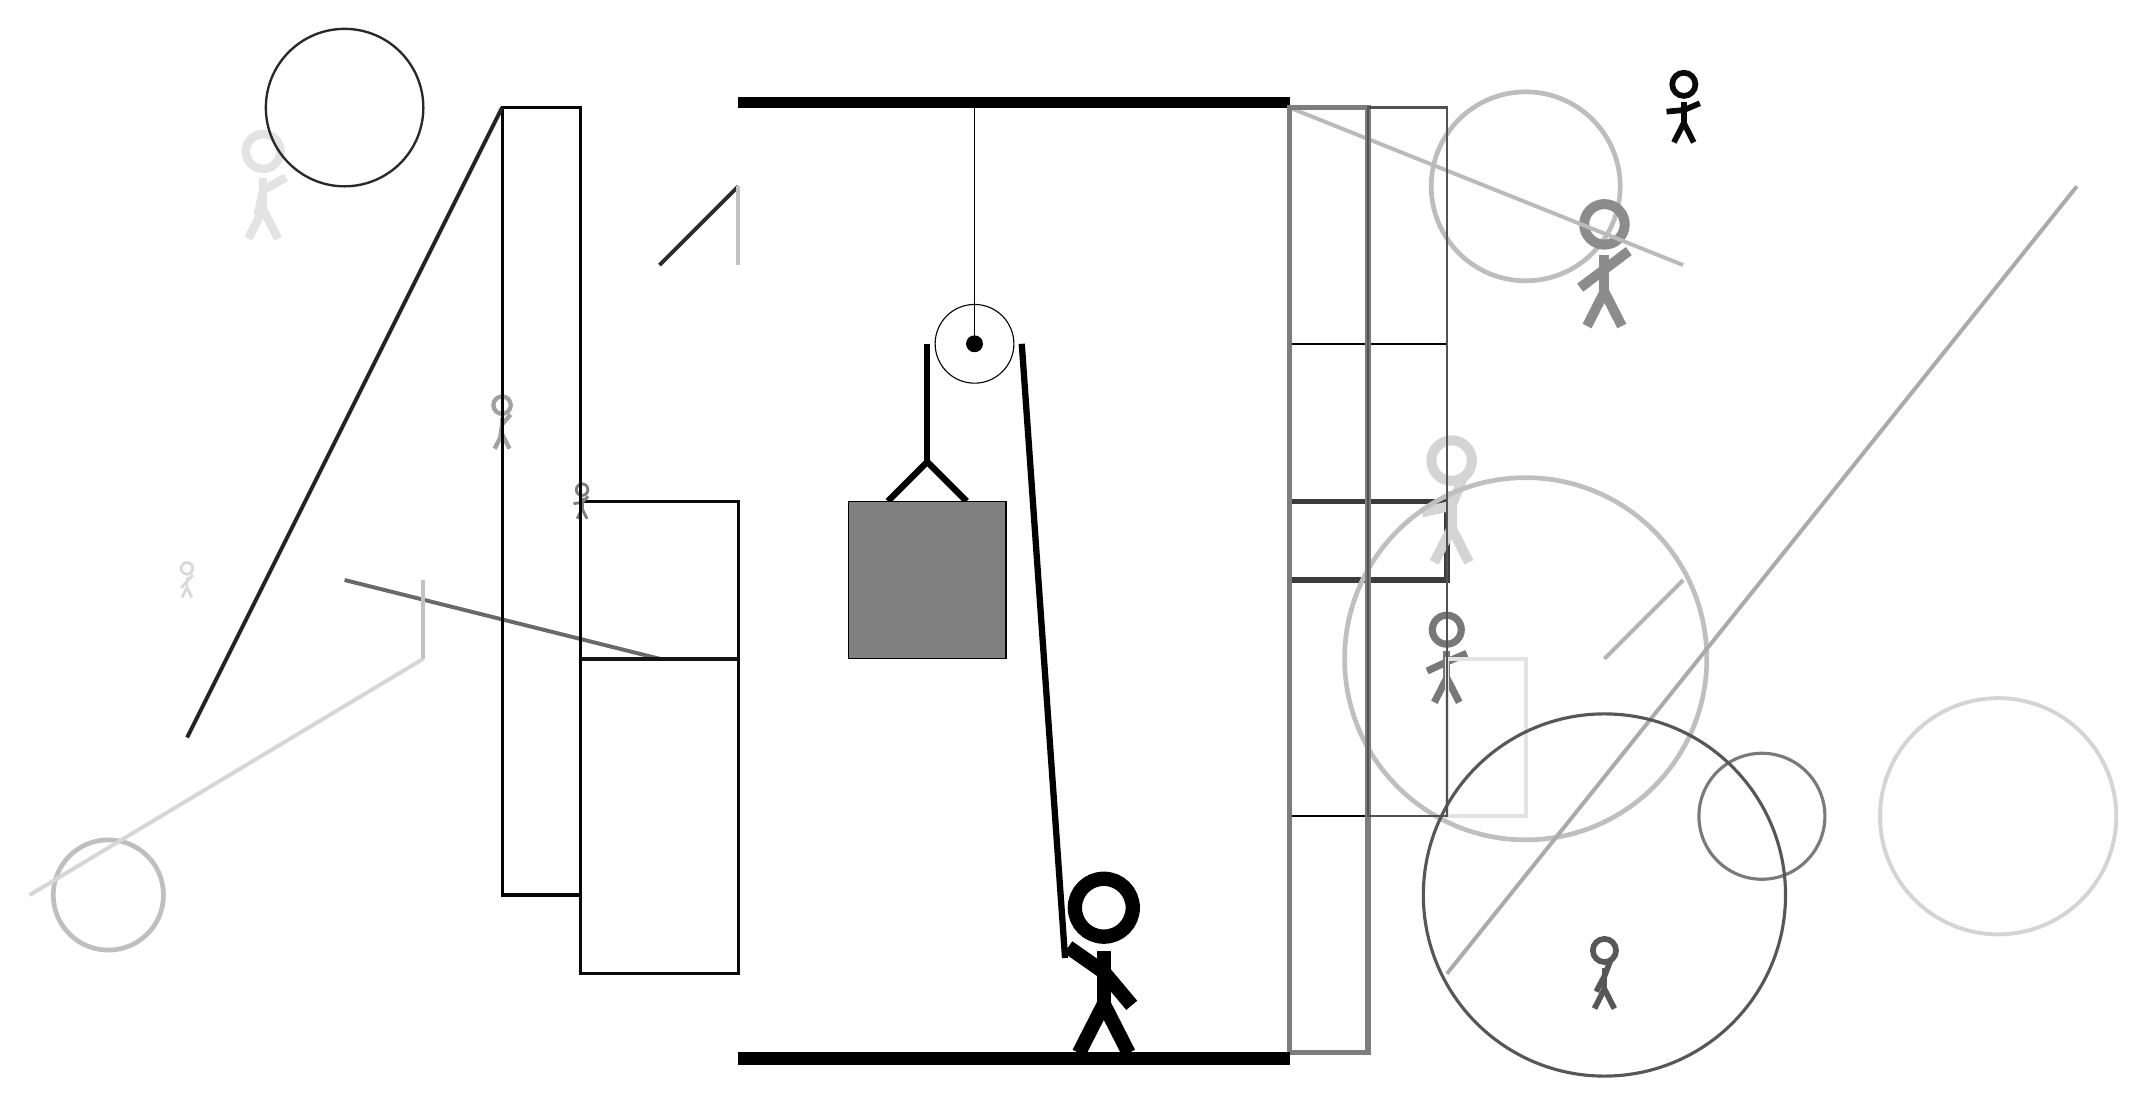
\begin{tikzpicture}
			%%%%% START %%%%%
			
			\draw[fill=black] (-2, 9) rectangle (5, 9.125);
			
			\draw (1, 6) circle (0.5);
			\draw[fill=black] (1, 6) circle (0.1);
			\draw (1, 9) -- (1, 6);
			
			\draw[line width=0.8mm] (-0.1, 4.0) -- (0.4, 4.5) -- (0.9, 4.0);
			\draw[fill=black!50] (-0.6, 4.0) rectangle (1.4, 2.0);
			
			\draw[line width=0.8mm] (0.4, 6) -- (0.4, 4.5);
			\centerarc[line width=0.8mm](1, 6)(0:180:0.6);
			\draw[line width=0.8mm](1.6, 6) -- (2.15, -1.8);
			
			\draw[line width=0.7mm, color=black!77] (7, 4) rectangle (5, 3);
			
			\node[line width=0.5mm, color=black!15] at (-9, 3) {\Strichmaxerl[2][50][45]};
			\node[line width=0.2mm, color=black!53] at (7, 2) {\Strichmaxerl[5][25][23]};
			\draw [line width=0.6mm, color=black!26](8, 8) circle (1.2);
			\draw[line width=0.5mm, color=black!11] (7, 2) rectangle (8, 0);
			
			\draw [line width=0.6mm, color=black!25](-10, -1) circle (0.7);
			\node[line width=0.5mm, color=black!96] at (10, 9) {\Strichmaxerl[4][5][23]};
			\draw[line width=0.5mm, color=black!82](-3, 7) -- (-2, 8);
			\draw[line width=0.5mm, color=black!59](-7, 3) -- (-3, 2);
			\node[line width=0.5mm, color=black!37] at (-5, 5) {\Strichmaxerl[3][82][49]};
			
			\node[line width=0.6mm, color=black!45] at (9, 7) {\Strichmaxerl[7][37][37]};
			\draw[line width=0.5mm, color=black!23](-2, 8) -- (-2, 7);
			\node[line width=0.7mm, color=black!17] at (7, 4) {\Strichmaxerl[7][13][68]};
			\draw[line width=0.4mm, color=black!96] (-2, 4) rectangle (-4, -2);
			\draw[line width=0.5mm, color=black!29](10, 3) -- (9, 2);
			\draw[line width=0.5mm, color=black!27](10, 7) -- (5, 9);
			\node[line width=0.3mm, color=black!51] at (-4, 4) {\Strichmaxerl[2][7][46]};
			
			\node[line width=0.6mm, color=black!11] at (-8, 8) {\Strichmaxerl[6][78][29]};
			\draw[line width=0.4mm, color=black!98] (-4, 9) rectangle (-5, -1);
			\draw[line width=0.5mm, color=black!92](-2, 2) -- (-4, 2);
			\draw [line width=0.5mm, color=black!17](14, 0) circle (1.5);
			
			\draw[line width=0.2mm, color=black!100] (5, 6) rectangle (7, 0);
			\draw [line width=0.6mm, color=black!25](8, 2) circle (2.3);
			\draw[line width=0.5mm, color=black!33](7, -2) -- (15, 8);
			\node[line width=0.4mm, color=black!66] at (9, -2) {\Strichmaxerl[4][62][69]};
			
			\draw [line width=0.3mm, color=black!84](-7, 9) circle (1.0);
			
			\draw[line width=0.5mm, color=black!16](-6, 2) -- (-11, -1);
			\draw [line width=0.4mm, color=black!52](11, 0) circle (0.8);
			\draw [line width=0.4mm, color=black!66](9, -1) circle (2.3);
			\draw[line width=0.7mm, color=black!51] (6, -3) rectangle (5, 9);
			\draw[line width=0.3mm, color=black!68] (7, 0) rectangle (6, 9);
			
			\draw[line width=0.5mm, color=black!86](-5, 9) -- (-9, 1);
			\draw[line width=0.5mm, color=black!24](-6, 2) -- (-6, 3);
			
			\node at (2.6, -1.9) {\Strichmaxerl[10][-35][-50]};
			
			\draw[fill=black] (-2, -3) rectangle (5, -3.15);
			
			%%%%% END %%%%%
		\end{tikzpicture}
	\end{figure}	
\end{document}